%==============================================================================
% Chapitre 47 - Désignation des cartouches
%==============================================================================

\section{Introduction}

Les cartouches sont désignées selon des conventions qui varient selon les
époques, les pays et les fabricants.

Certaines désignations paraissent intuitives tandis que d'autres semblent
particulièrement énigmatiques.

Comprendre ces appellations permet d'identifier rapidement les principales
caractéristiques d'une munition.

\begin{aretenir}

La désignation d'une cartouche fournit souvent des informations utiles mais
ne décrit pas toujours exactement ses dimensions réelles.

\end{aretenir}

\section{Pourquoi une désignation ?}

Des milliers de cartouches différentes ont été développées au cours de
l'histoire.

Une désignation normalisée permet notamment :

\begin{itemize}
    \item d'identifier une cartouche ;
    \item d'éviter les confusions ;
    \item de garantir la compatibilité des armes ;
    \item de faciliter les échanges techniques.
\end{itemize}

\section{Le système métrique}

De nombreuses cartouches utilisent une désignation de la forme :

\begin{equation}
A \times B
\end{equation}

où :

\begin{itemize}
    \item $A$ représente généralement le calibre nominal ;
    \item $B$ représente généralement la longueur de l'étui.
\end{itemize}

\section{Exemple : 9×19 mm}

La cartouche 9×19 mm possède :

\begin{itemize}
    \item un calibre nominal de 9 mm ;
    \item un étui d'environ 19 mm de longueur.
\end{itemize}

Elle est également connue sous le nom :

\begin{quote}
9 mm Parabellum
\end{quote}

ou :

\begin{quote}
9 mm Luger.
\end{quote}

\section{Exemple : 5,56×45 mm}

La cartouche 5,56×45 mm possède :

\begin{itemize}
    \item un calibre nominal de 5,56 mm ;
    \item un étui d'environ 45 mm.
\end{itemize}

Elle est largement utilisée dans les fusils d'assaut modernes.

\begin{figure}[htbp]
\centering

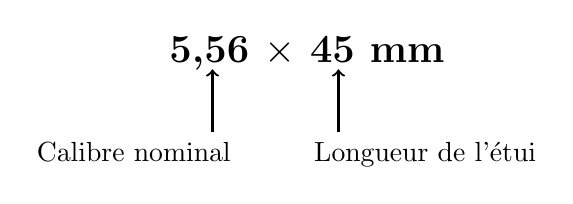
\begin{tikzpicture}[scale=1]

\node[font=\Large\bfseries] (cart) at (0,0)
{5,56 $\times$ 45 mm};

\draw[->,thick]
(-1.2,-1)
--
(-1.2,-0.2);

\node[below]
at (-2.2,-1)
{Calibre nominal};

\draw[->,thick]
(0.4,-1)
--
(0.4,-0.2);

\node[below]
at (1.5,-1)
{Longueur de l'étui};

\end{tikzpicture}

\caption{Exemple de décomposition d'une désignation métrique.}
\label{fig:designation_metrique}

\end{figure}

\section{Exemple : 7,62×51 mm}

La cartouche 7,62×51 mm possède :

\begin{itemize}
    \item un calibre nominal de 7,62 mm ;
    \item un étui d'environ 51 mm.
\end{itemize}

Elle est notamment connue dans sa version civile :

\begin{quote}
.308 Winchester
\end{quote}

bien que les deux cartouches ne soient pas strictement identiques dans tous
les contextes.

\section{Le système impérial}

Dans les pays anglo-saxons, les désignations utilisent souvent le pouce.

On rencontre ainsi :

\begin{itemize}
    \item .22 ;
    \item .30 ;
    \item .308 ;
    \item .357 ;
    \item .45.
\end{itemize}

Le point décimal indique une fraction de pouce.

\section{Exemple : .308 Winchester}

Dans cette désignation :

\begin{itemize}
    \item .308 indique le diamètre nominal du projectile en pouce ;
    \item Winchester désigne l'entreprise ayant développé ou popularisé la
          cartouche.
\end{itemize}

\section{Exemple : .45 ACP}

La désignation ACP signifie :

\begin{quote}
Automatic Colt Pistol
\end{quote}

Le nom fait référence à l'origine historique de la cartouche.

\section{Exemple : .44 Magnum}

Dans certains cas, la désignation comporte un nom commercial.

Le terme Magnum est historiquement associé à des cartouches offrant des
performances supérieures à celles de versions antérieures apparentées.

\section{Exemple : .30-06 Springfield}

Cette désignation est souvent source d'interrogations.

Elle signifie :

\begin{itemize}
    \item .30 : calibre nominal en pouce ;
    \item 06 : année d'adoption 1906 ;
    \item Springfield : référence à l'arsenal associé à son développement.
\end{itemize}

\begin{figure}[htbp]
\centering

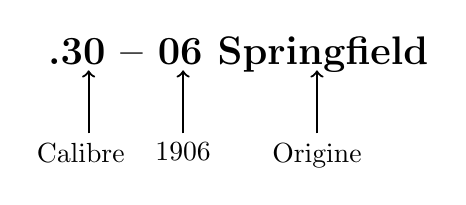
\begin{tikzpicture}[scale=1]

\node[font=\Large\bfseries]
(cart)
at (0,0)
{.30 -- 06 Springfield};

\draw[->,thick]
(-1.9,-1)
--
(-1.9,-0.2);

\node[below]
at (-2,-1)
{Calibre};

\draw[->,thick]
(-0.7,-1)
--
(-0.7,-0.2);

\node[below]
at (-0.7,-1)
{1906};

\draw[->,thick]
(1,-1)
--
(1,-0.2);

\node[below]
at (1,-1)
{Origine};

\end{tikzpicture}

\caption{Exemple de décomposition d'une désignation historique.}
\label{fig:designation_3006}

\end{figure}

\section{Les désignations historiques}

Certaines désignations anciennes reflètent des conventions aujourd'hui
abandonnées.

On peut rencontrer des références liées :

\begin{itemize}
    \item à la masse du projectile ;
    \item à la charge de poudre ;
    \item à l'année d'adoption ;
    \item au fabricant.
\end{itemize}

\section{Le rôle des fabricants}

De nombreux fabricants ont développé leurs propres cartouches.

Le nom du fabricant est souvent conservé dans la désignation :

\begin{itemize}
    \item Winchester ;
    \item Remington ;
    \item Weatherby ;
    \item Norma ;
    \item Lapua.
\end{itemize}

\section{Les désignations militaires}

Les organisations militaires utilisent parfois des désignations spécifiques.

Une même cartouche peut ainsi posséder :

\begin{itemize}
    \item une désignation civile ;
    \item une désignation militaire ;
    \item une référence normalisée.
\end{itemize}

\section{Normalisation}

Afin d'éviter toute ambiguïté, plusieurs organismes définissent des normes.

Ces normes précisent notamment :

\begin{itemize}
    \item les dimensions ;
    \item les tolérances ;
    \item les pressions admissibles ;
    \item les méthodes d'essai.
\end{itemize}

\section{Pourquoi les désignations sont-elles parfois trompeuses ?}

Les appellations historiques ont souvent été conservées malgré les évolutions
techniques.

Par conséquent :

\begin{itemize}
    \item certaines dimensions sont approximatives ;
    \item certaines valeurs sont arrondies ;
    \item certaines désignations ne correspondent plus exactement aux mesures
          réelles.
\end{itemize}

\section{Comment identifier une cartouche ?}

Pour identifier correctement une cartouche, il est souvent nécessaire de
connaître :

\begin{itemize}
    \item son calibre ;
    \item sa longueur d'étui ;
    \item sa désignation complète ;
    \item son éventuelle normalisation.
\end{itemize}

Le calibre seul est rarement suffisant.

\section{Vers les pressions nominales}

Deux cartouches de dimensions voisines peuvent présenter des pressions très
différentes.

L'étude des pressions nominales constitue donc l'étape suivante dans la
compréhension des munitions modernes.

\section{À retenir}

\begin{aretenir}

\begin{itemize}
    \item Les désignations de cartouches suivent plusieurs conventions.
    \item Les systèmes métrique et impérial coexistent.
    \item Certaines désignations reflètent des caractéristiques techniques.
    \item D'autres sont principalement historiques ou commerciales.
    \item Le calibre seul ne permet pas d'identifier précisément une
          cartouche.
\end{itemize}

\end{aretenir}

\begin{figure}[htbp]
\centering

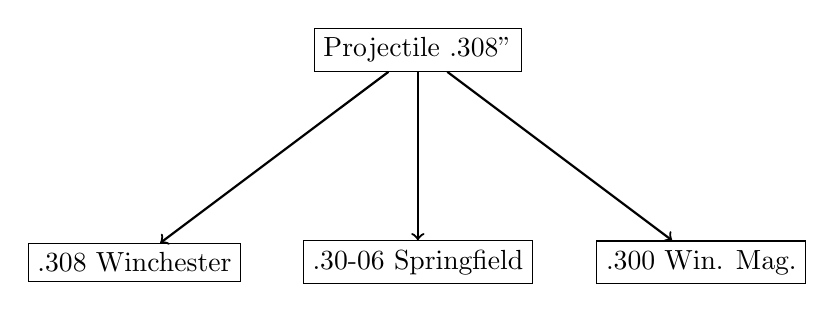
\begin{tikzpicture}[scale=0.9]

% Projectile commun
\node[draw,minimum width=2.5cm]
(P)
at (0,0)
{Projectile .308"};

% Cartouches
\node[draw]
(A)
at (-4,-3)
{.308 Winchester};

\node[draw]
(B)
at (0,-3)
{.30-06 Springfield};

\node[draw]
(C)
at (4,-3)
{.300 Win. Mag.};

\draw[->,thick] (P) -- (A);
\draw[->,thick] (P) -- (B);
\draw[->,thick] (P) -- (C);

\end{tikzpicture}

\caption{Un même diamètre de projectile peut être utilisé dans plusieurs cartouches différentes.}
\label{fig:famille_308}

\end{figure}

\begin{table}[htbp]
\centering
\caption{Exemples de désignations de cartouches.}
\label{tab:designations}

\begin{tabular}{lll}
\hline
Désignation & Système & Signification principale \\
\hline
9×19 mm & Métrique & calibre + longueur d'étui \\
5,56×45 mm & Métrique & calibre + longueur d'étui \\
7,62×51 mm & Métrique & calibre + longueur d'étui \\
.308 Winchester & Impérial & calibre + fabricant \\
.30-06 Springfield & Historique & calibre + année + origine \\
.45 ACP & Impérial & calibre + usage historique \\
\hline
\end{tabular}

\end{table}
